\documentclass[9pt,aspectratio=169]{beamer}
\mode<presentation>
\usepackage[T1]{fontenc}
\usepackage{color}
\usepackage{graphicx}
\usepackage{natbib}
\usepackage{listings}
\usepackage{booktabs}

\definecolor{codegreen}{rgb}{0,0.6,0}
\definecolor{codegray}{rgb}{0.5,0.5,0.5}
\definecolor{codepurple}{rgb}{0.58,0,0.82}
\definecolor{backcolour}{rgb}{0.95,0.95,0.92}

\lstdefinestyle{mystyle}{
	backgroundcolor=\color{backcolour},   
	commentstyle=\color{codegreen},
	keywordstyle=\color{magenta},
	numberstyle=\tiny\color{codegray},
	stringstyle=\color{codepurple},
	basicstyle=\ttfamily\footnotesize,
	breakatwhitespace=false,         
	breaklines=true,                 
	captionpos=b,                    
	keepspaces=true,                 
	numbers=left,                    
	numbersep=5pt,                  
	showspaces=false,                
	showstringspaces=false,
	showtabs=false,                  
	tabsize=2
}

\lstset{style=mystyle}

\usepackage{hyperref}

\usetheme{Singapore}
%\usecolortheme{seahorse}

\usefonttheme{professionalfonts}

\title[LLM screening]{Can Zero-shot LLMs save additional work in machine learning prioritised screening for systematic reviews?}

\author{Max Callaghan}
\institute[MCC]{

\includegraphics[height=1cm,width=2cm]{images/MCC_Logo_RZ_rgb.jpg}
}



\newtheorem*{remark}{}

\bibliographystyle{apalike}

\begin{document}

\begin{frame}
\titlepage
\end{frame}


%\section{Introduction}
%
%\section{Implementation}

\section{Introduction}

\begin{frame}{Can LLMs help us to save more work?}
	
\begin{columns}
	\begin{column}{0.5\linewidth}
		\begin{itemize}
			\item<1->Prioritised screening has saved us a lot of work
			\item<2->But we still spend substantial amounts of time screening documents for systematic reviews
			\item<3->LLMs have been proposed as a solution, with
			\begin{itemize}
				\item<4-> \cite{wang_zero-shot_2024} showing impressive results for the zero-shot setting
				\item<5-> and  \cite{xia_llmscreen_2024} erroneously claiming that LLMs fix all of the problems faced until now by ml+screening
			\end{itemize} 
			\item<6-> There are a lot of bad papers, which will continue to proliferate, each tweaking some parameters to achieve a high performance that cannot be generalised
		\end{itemize}
	\end{column}

	\begin{column}{0.5\linewidth}
		\only<4>{
		\begin{figure}
			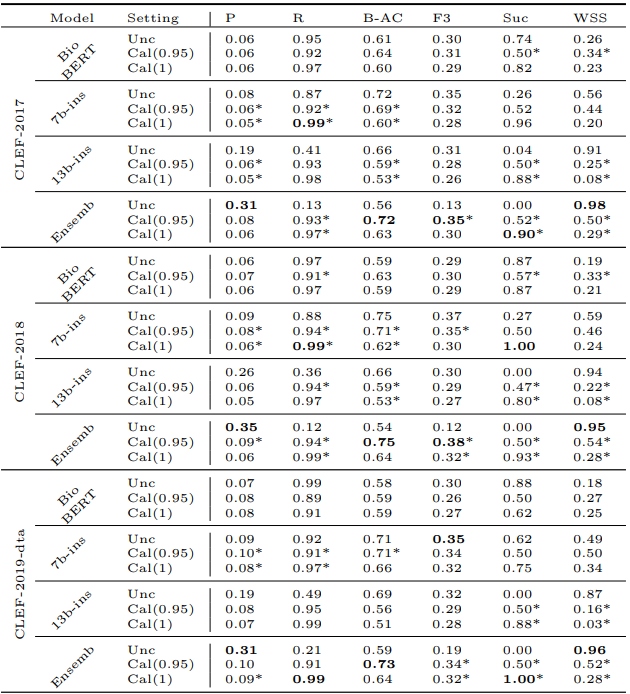
\includegraphics[width=\columnwidth]{images/tab3-1}
		\end{figure}
		}	
		\only<5->{
					\begin{figure}
				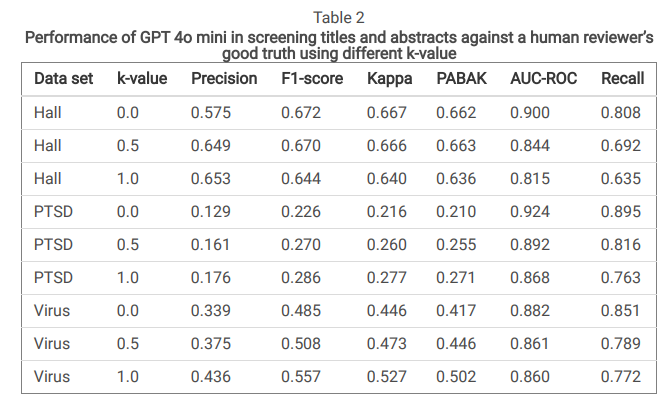
\includegraphics[width=\columnwidth]{images/xia}
			\end{figure}
	}
	\end{column}
\end{columns}

\end{frame}

\begin{frame}{Realistic and useful evaluations of LLMs for screening}
	
	Despite the hype, LLMs might still be helpful, but we need to know
	
	\begin{itemize}
		\item<2->How do LLMs compare against commonly used (and much cheaper!) baselines?
		\item<3->How could they safely be used in the real world (Hint: with stopping criteria and prioritised screening)
	\end{itemize}
\end{frame}

\section{Prioritisation with LLMs}

\begin{frame}{Zero-shot Generative Large Language Models for Systematic Review Screening Automation}
	
	\cite{wang_zero-shot_2024} propose a method to extract probability-like scores from LLMs for inclusion/exclusion decisions in a systematic review
	
	\begin{figure}
		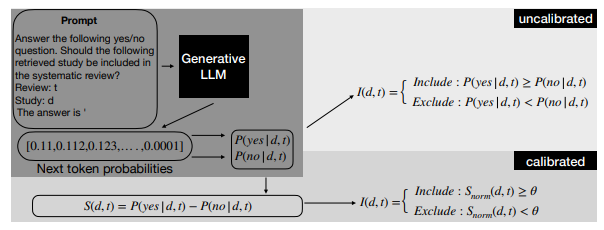
\includegraphics[width=\columnwidth]{images/fig1}
	\end{figure}
\end{frame}


\begin{frame}[fragile]{Implementation is relatively straightforward}
\small
\begin{lstlisting}[language=Python]
def binary_probs(tokenizer, model, prompt, no_words=['no'], yes_words=['yes'], return_all=False):
    device = 'cuda' if torch.cuda.is_available() else 'cpu'
    encoded_text = tokenizer(prompt, return_tensors="pt").to(device)
    #1. step to get the logits of the next token
    with torch.inference_mode():
        outputs = model(**encoded_text)

    next_token_logits = outputs.logits[0, -1, :]

    # 2. step to convert the logits to probabilities
    next_token_probs = torch.softmax(next_token_logits, -1)

    topk_next_tokens= torch.topk(next_token_probs, 50)
    tokens = [tokenizer.decode(x).strip().lower() for x in topk_next_tokens.indices]
    p = topk_next_tokens.values

    df = pd.DataFrame.from_dict({'t': tokens,'p': p.cpu()})
    y = df[df['t'].isin(yes_words)]['p'].sum()
    n = df[df['t'].isin(no_words)]['p'].sum()

    if return_all:
        return df.groupby('t').sum().reset_index().sort_values('p', ascending=False).reset_index(drop=True)
    return y-n, y+n
\end{lstlisting}

\end{frame}

\begin{frame}[fragile]{Implementation is relatively straightforward}
	

	\small
\begin{lstlisting}[language=Python]
prompt = Template('''<s>[INST] <<SYS>>
You are a systematic review helper tasked with finding out whether a study is relevant to the review $t

Answer 'yes' if the study is relevant, or 'no' if not
<</SYS>>

Study: $s 

Should the study be included? Answer yes or no. [/INST] ''')

prompt.substitute({'t': review, 's': study_title}),
\end{lstlisting}


\end{frame}



\begin{frame}[fragile]{Implementation is relatively straightforward}

	\begin{columns}
	\begin{column}{0.5\linewidth}
		\begin{figure}
			\footnotesize
			%\includegraphics[width=\linewidth]{images/example.txt}
			\input{images/example.txt}
		\end{figure}
	\end{column}
	\begin{column}{0.5\linewidth}
		\only<2->{\begin{figure}
				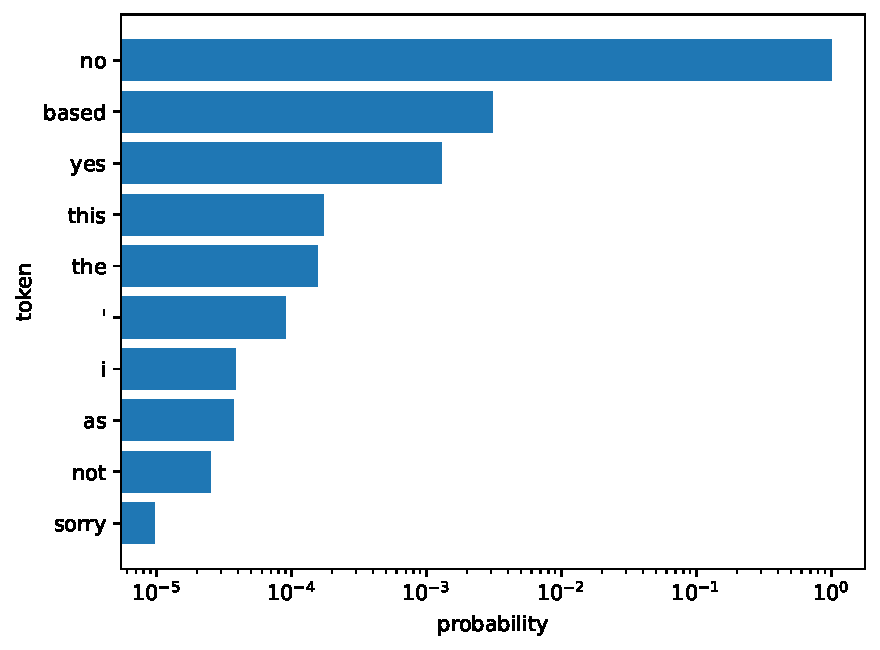
\includegraphics[width=\columnwidth]{images/example_probs.pdf}
		\end{figure}}
	\end{column}
\end{columns}

	
\end{frame}

\section{Comparison}

\begin{frame}{Comparing priorisation approaches}

\begin{itemize}
	\item<1-> We evaluate using the Synergy dataset \cite{de_bruin_synergy_2023} of 26 systematic reviews (Tim, Diana, Sergio, Lena, and James, will make a much bigger one!)
	\item<2-> For each review, we generate 100 different initial random samples of 10\%, and do normal prioritised screening in batches of 10\% with an SVM 100 times
	\item<3-> We also make a prediction for each document with 4 Llama models of different sizes and ages
	\item<4-> We turn these predictions into a prioritised list of documents to be screened
\end{itemize}
	
\end{frame}


\section{Results}

\begin{frame}{Result \#1: It works!}
	\begin{columns}
		\begin{column}{0.4\linewidth}
			\begin{itemize}
				\item<1-> The method produces a ranking that identifies all relevant documents before all documents have been screened
				\item<2-> The first model we tried was much worse than our SVM, but newer and bigger models were much more promising!
				\item<3-> But performance varied across datasets
				\item<4-> ROC AUC scores offer one way to compare rankings
			\end{itemize}
		\end{column}
		\begin{column}{0.6\linewidth}
			\only<1>{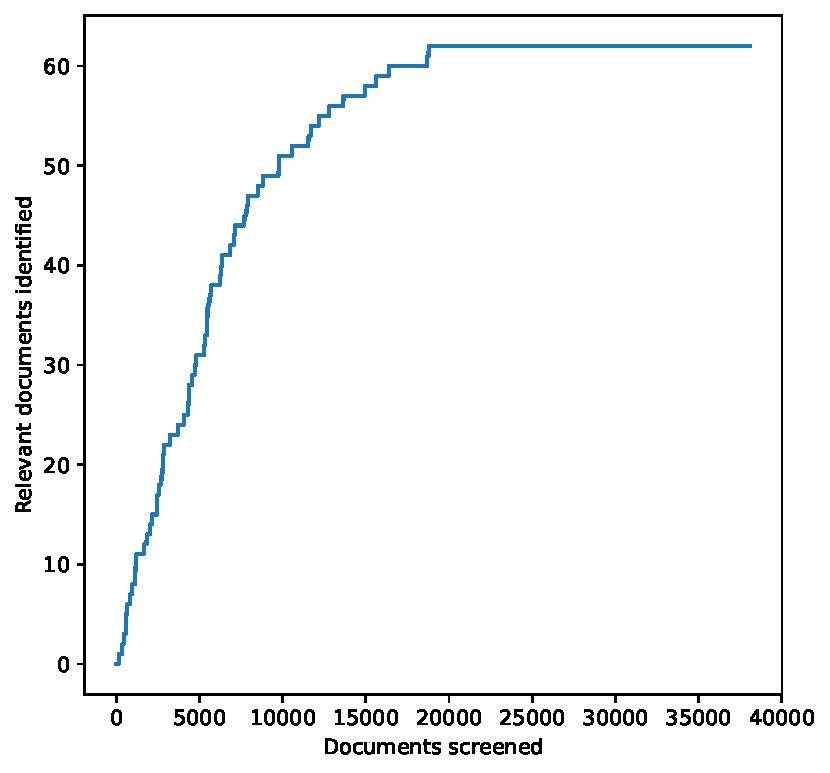
\includegraphics[width=\linewidth]{../../figures/LLM_Brouwer_simple.pdf}}
			\only<2>{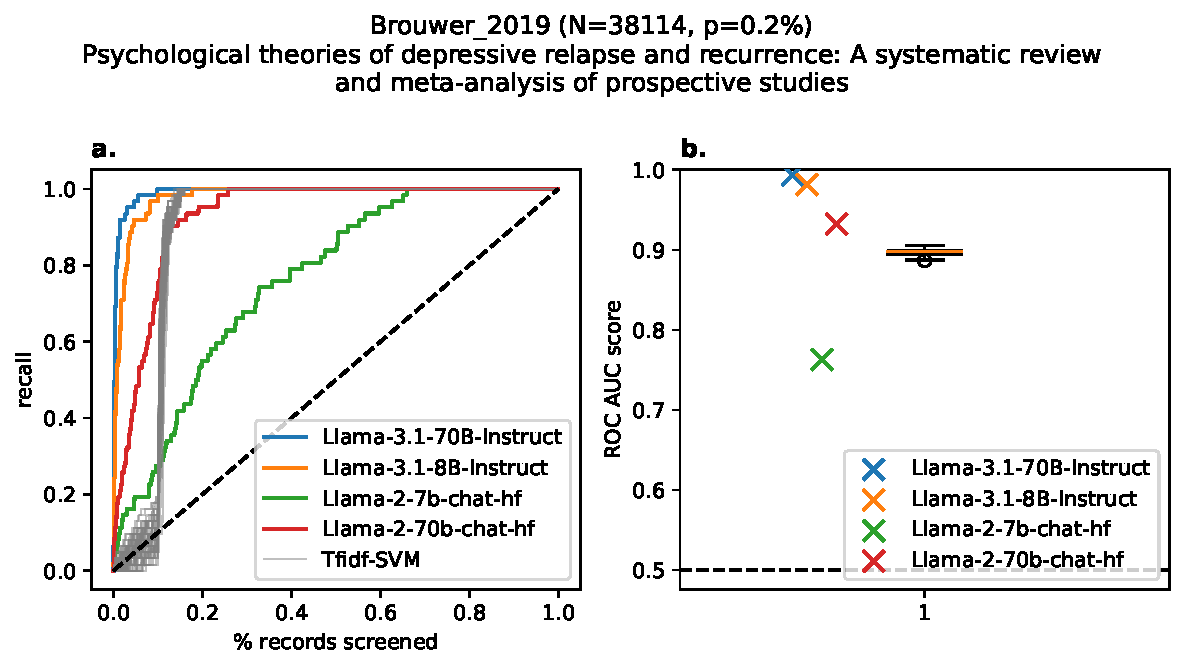
\includegraphics[width=\linewidth]{../../figures/Brouwer_2019.pdf}}
				\only<3>{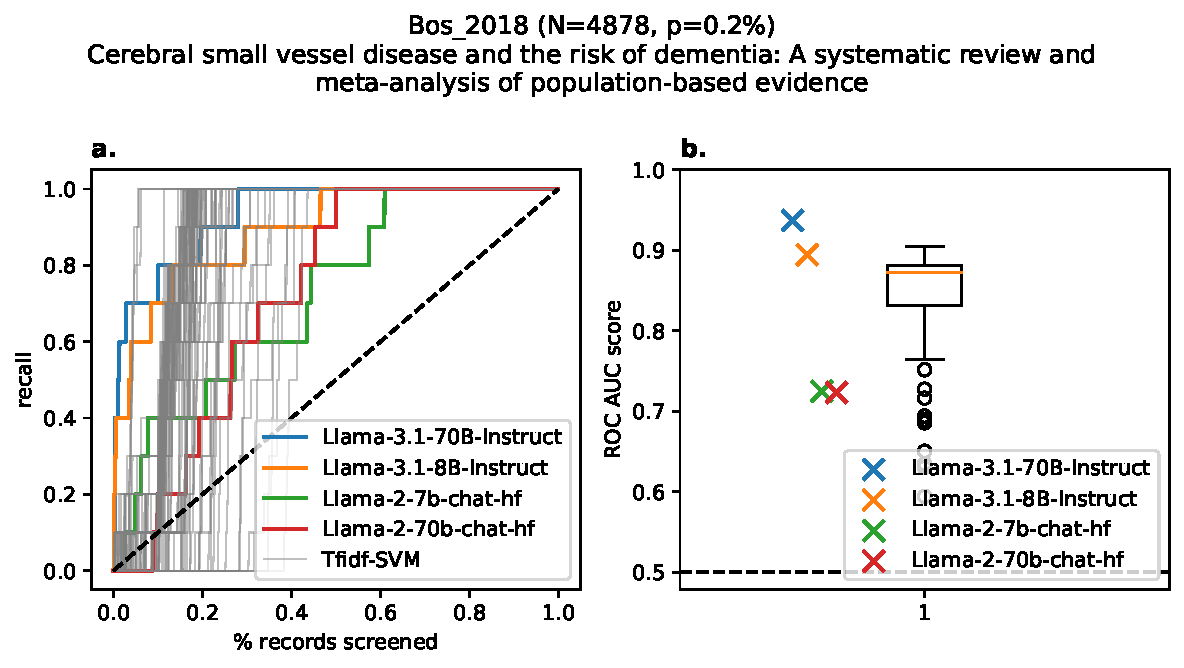
\includegraphics[width=\columnwidth]{../../figures/Bos_2018.pdf}}
				\only<4>{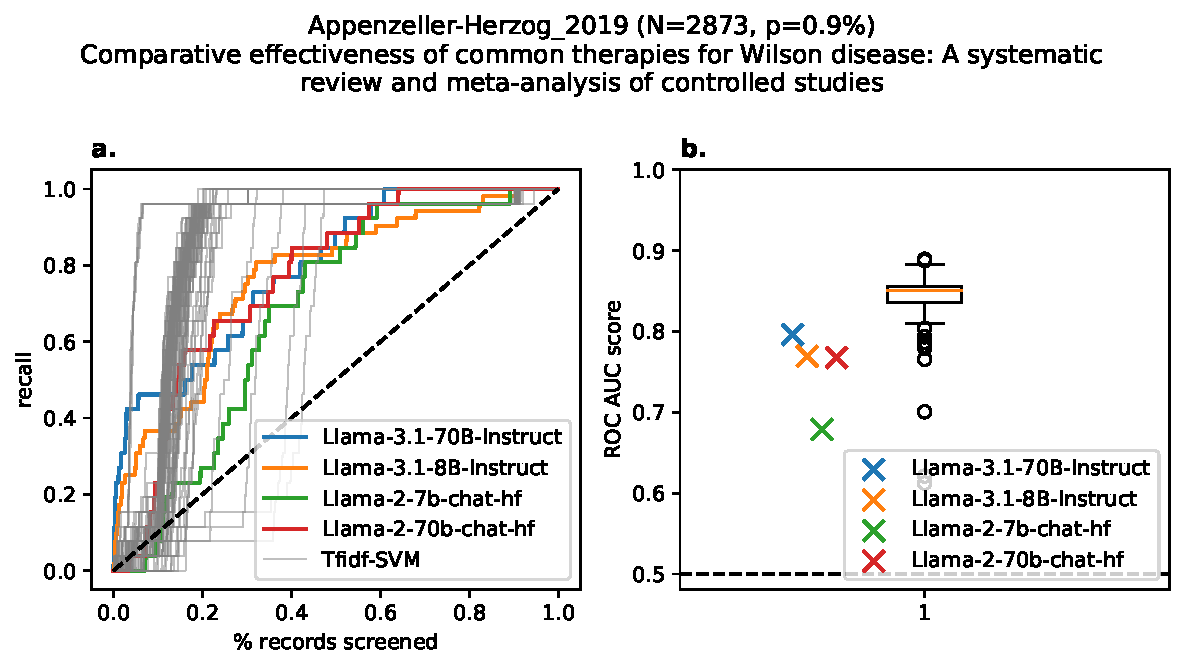
\includegraphics[width=\columnwidth]{../../figures/Appenzeller-Herzog_2019.pdf}}
			\only<5>{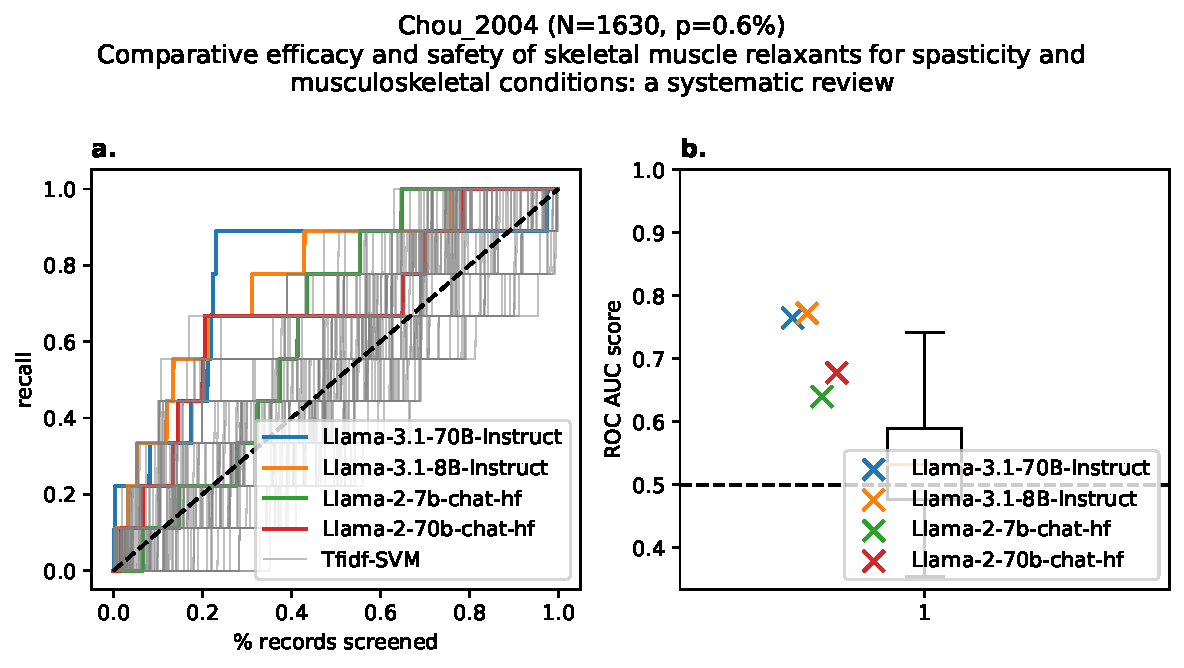
\includegraphics[width=\columnwidth]{../../figures/Chou_2004.pdf}}
			\only<6>{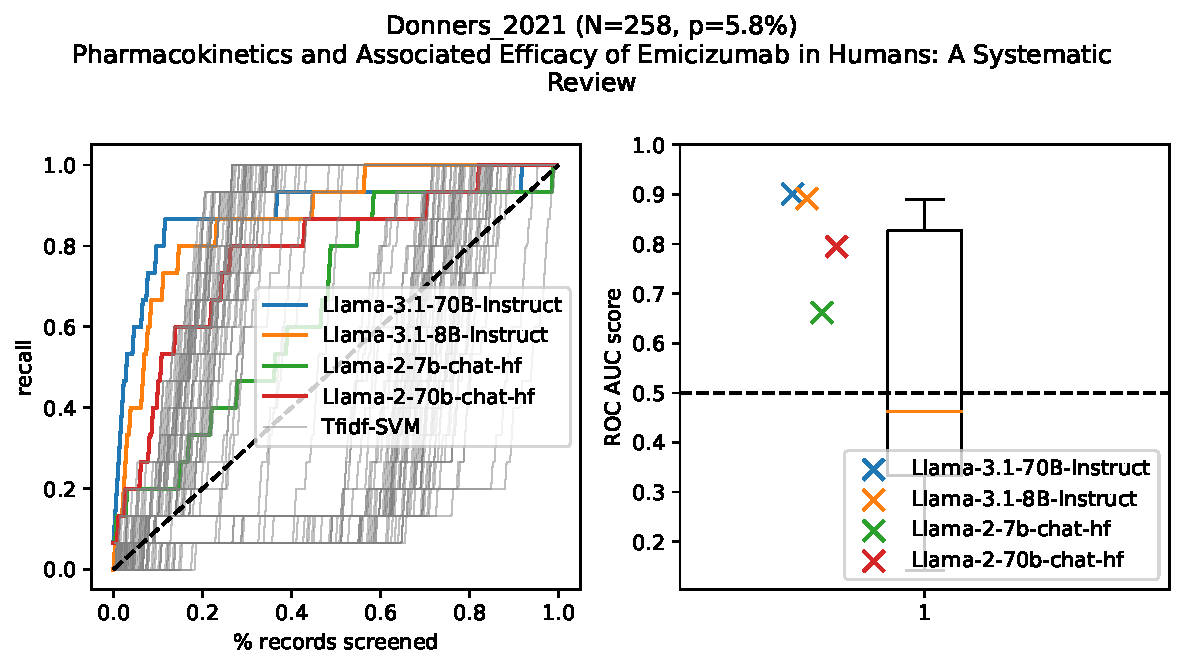
\includegraphics[width=\columnwidth]{../../figures/Donners_2021.pdf}}
			\only<7>{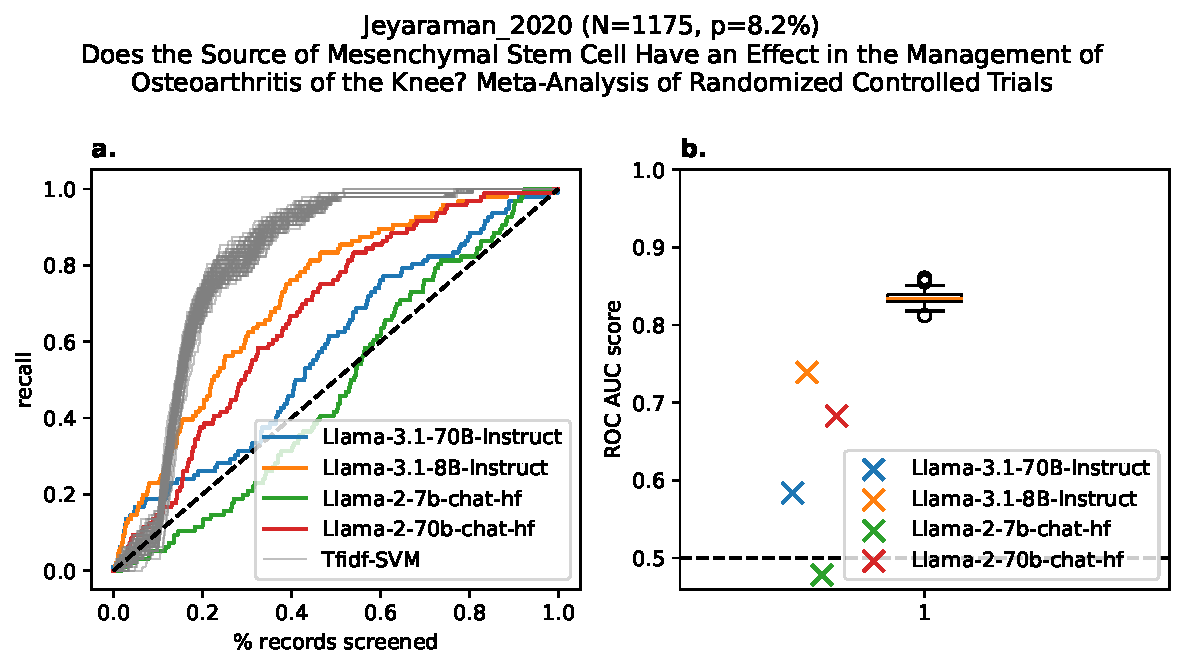
\includegraphics[width=\columnwidth]{../../figures/Jeyaraman_2020.pdf}}
			\only<8>{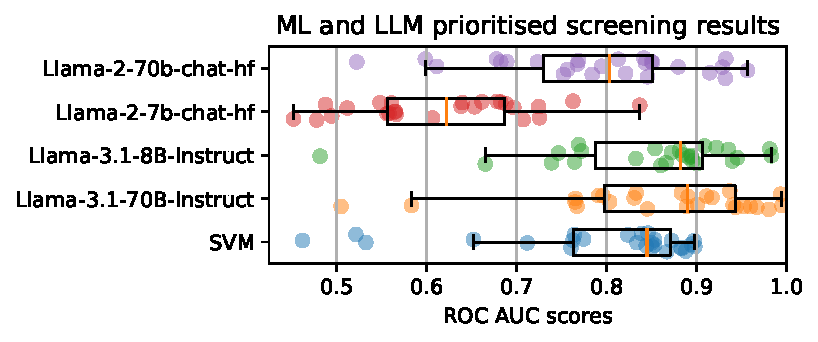
\includegraphics[width=\columnwidth]{../../figures/macro_comparison.pdf}}
			%\only<3>{}
		\end{column}
	\end{columns}
\end{frame}


%\begin{frame}{All results}
%	\begin{columns}
%	\begin{column}{0.618\linewidth}
%		\begin{figure}
%			
%			\only<1->{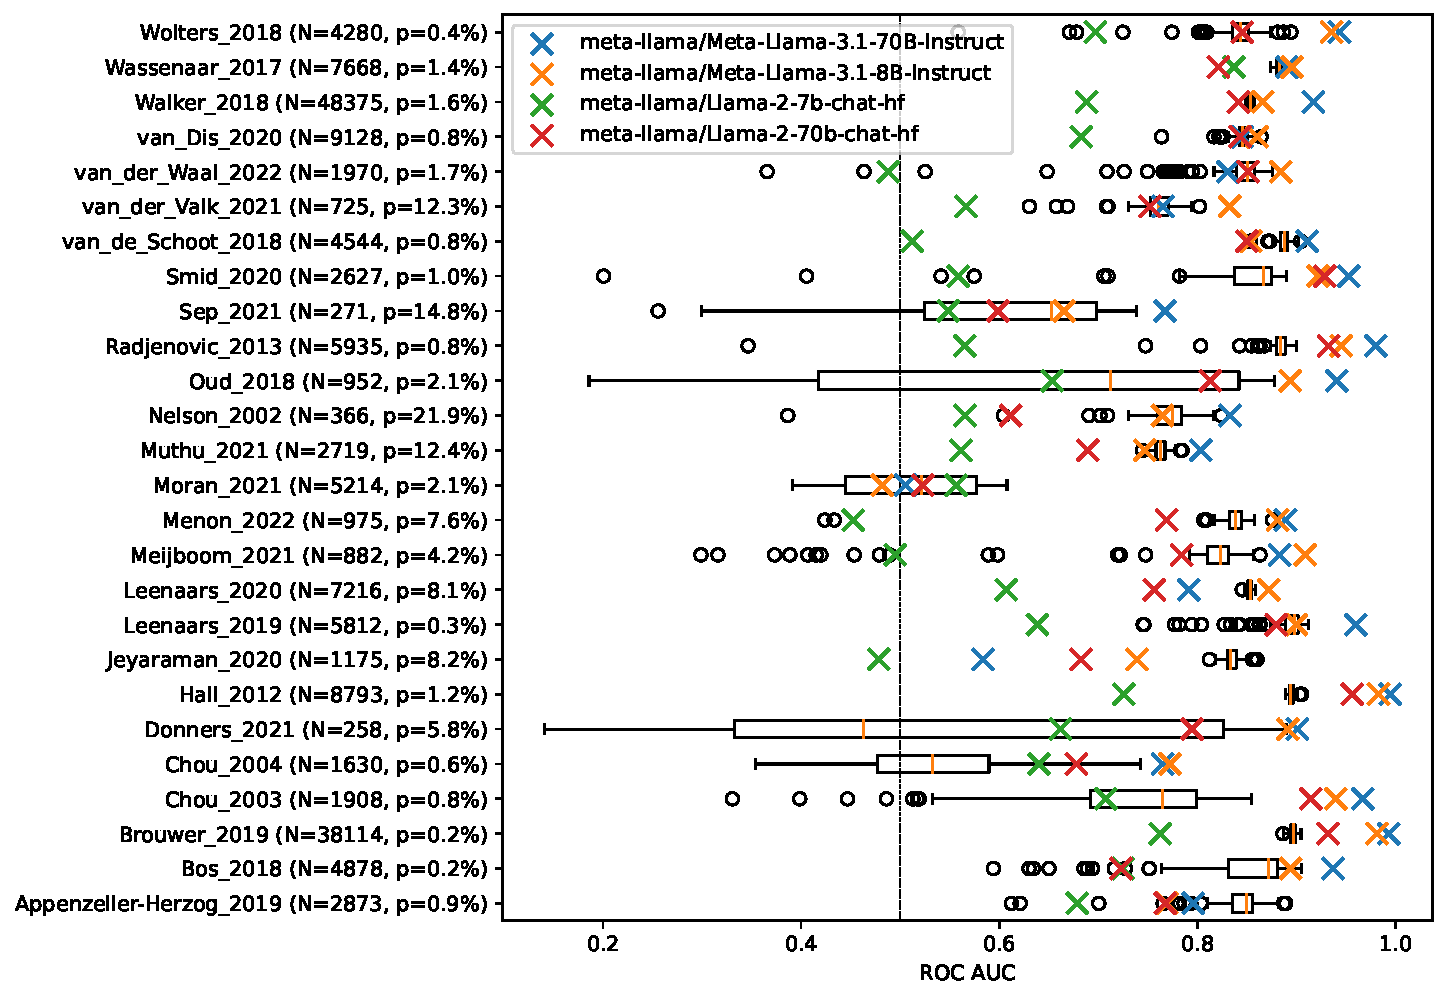
\includegraphics[width=\columnwidth]{../../figures/llm_svm_roc.pdf}}
%
%		\end{figure}
%	\end{column}
%	\begin{column}{0.382\linewidth}
%		\begin{itemize}
%			\item<1-> LLMs and basic active learning pipelines seem to have different weakneses
%			\item<2-> Combining both could improve general performance
%			\item<3-> LLMs seem most useful for smaller datasets (where active learning has little time to learn)
%		\end{itemize}
%	\end{column}
%\end{columns}
%\end{frame}

\begin{frame}{Stopping criteria}
	\begin{columns}
		\begin{column}{0.32\linewidth}
			\begin{itemize}
				\item<1->Next, we calculate scores for our stopping criteria with a range of different recall targets
				\item<2->Stopping when $p<\alpha$ gives a recall > target in the $\alpha^{th}$ percentile, in 97/100 settings
				\item<3->In most settings, total work savings were greater for SVMs 
			\end{itemize}
		\end{column}
		\begin{column}{0.68\linewidth}
			\only<2>{
			\begin{table}
				\scriptsize
				\begin{tabular}{llrrrrr}
\toprule
 & model & SVM & Llama-2-7b & Llama-2-70b & Llama-3.1-8B & Llama-3.1-70B \\
r target & confidence &  &  &  &  &  \\
\midrule
0.80 & 0.50 & 0.938 & \textbf{0.758} & 0.893 & 0.911 & 0.911 \\
 & 0.80 & 0.924 & \textbf{0.797} & 0.866 & 0.845 & 0.889 \\
 & 0.90 & 0.900 & 0.818 & 0.872 & 0.836 & 0.876 \\
 & 0.95 & 0.867 & 0.806 & 0.888 & 0.878 & 0.878 \\
 & 0.99 & 0.811 & 0.838 & 0.865 & 0.876 & 0.886 \\
\cline{1-7}
0.90 & 0.50 & 0.963 & 0.905 & 0.936 & 0.957 & 0.954 \\
 & 0.80 & 0.957 & 0.900 & 0.958 & 0.961 & 0.933 \\
 & 0.90 & 0.947 & 0.937 & 0.959 & 0.953 & 0.939 \\
 & 0.95 & 0.933 & 0.943 & 0.944 & 0.947 & 0.939 \\
 & 0.99 & 0.928 & 0.941 & 0.947 & 0.926 & 0.958 \\
\cline{1-7}
0.95 & 0.50 & 0.979 & \textbf{0.947} & 1.000 & 0.981 & 0.987 \\
 & 0.80 & 0.974 & 0.973 & 0.976 & 0.975 & 0.979 \\
 & 0.90 & 0.973 & 0.968 & 0.981 & 0.978 & 0.980 \\
 & 0.95 & 0.964 & 0.973 & 0.982 & 0.976 & 0.968 \\
 & 0.99 & 0.973 & 0.975 & 0.986 & 0.983 & 0.975 \\
\cline{1-7}
0.99 & 0.50 & 1.000 & 1.000 & 1.000 & 1.000 & 1.000 \\
 & 0.80 & 0.994 & 1.000 & 1.000 & 1.000 & 0.991 \\
 & 0.90 & 0.993 & 0.996 & 1.000 & 0.999 & 0.996 \\
 & 0.95 & 0.993 & 0.997 & 1.000 & 0.999 & 0.996 \\
 & 0.99 & 0.996 & 0.992 & 0.999 & 0.997 & 0.996 \\
\cline{1-7}
\bottomrule
\end{tabular}


			\end{table}
		}
			\only<3>{
	\begin{table}
		\scriptsize
		\begin{tabular}{llrrrrr}
\toprule
 & model & SVM & Llama-2-7b & Llama-2-70b & Llama-3.1-8B & Llama-3.1-70B \\
r target & confidence &  &  &  &  &  \\
\midrule
0.80 & 0.50 & 126,898 & 100,248 & 121,777 & 127,401 & \textbf{132,808} \\
 & 0.80 & 113,708 & 64,568 & 97,147 & 111,411 & \textbf{114,748} \\
 & 0.90 & 105,053 & 57,678 & 90,327 & 101,871 & \textbf{106,668} \\
 & 0.95 & 98,503 & 48,608 & 83,338 & 94,921 & \textbf{101,288} \\
 & 0.99 & \textbf{87,803} & 37,838 & 71,397 & 79,471 & 85,058 \\
\cline{1-7}
0.90 & 0.50 & 114,988 & 65,778 & 99,217 & 112,011 & \textbf{115,498} \\
 & 0.80 & 93,923 & 42,768 & 79,807 & 83,661 & \textbf{97,438} \\
 & 0.90 & \textbf{84,658} & 34,158 & 65,007 & 76,701 & 82,268 \\
 & 0.95 & \textbf{76,483} & 28,748 & 59,447 & 69,251 & 73,108 \\
 & 0.99 & \textbf{62,350} & 23,118 & 49,790 & 55,091 & 59,088 \\
\cline{1-7}
0.95 & 0.50 & 98,258 & 44,408 & 82,907 & 94,731 & \textbf{101,318} \\
 & 0.80 & \textbf{74,098} & 27,238 & 58,587 & 64,281 & 68,678 \\
 & 0.90 & \textbf{63,245} & 21,738 & 44,470 & 53,091 & 57,388 \\
 & 0.95 & \textbf{54,860} & 18,781 & 37,370 & 45,954 & 48,671 \\
 & 0.99 & \textbf{41,676} & 13,545 & 27,171 & 34,855 & 35,592 \\
\cline{1-7}
0.99 & 0.50 & \textbf{63,573} & 22,638 & 42,897 & 54,811 & 55,378 \\
 & 0.80 & \textbf{31,323} & 11,158 & 20,597 & 29,191 & 30,398 \\
 & 0.90 & \textbf{21,160} & 5,825 & 13,480 & 13,641 & 18,478 \\
 & 0.95 & \textbf{16,229} & 4,065 & 8,837 & 9,435 & 11,938 \\
 & 0.99 & \textbf{7,980} & 1,985 & 4,355 & 4,934 & 6,625 \\
\cline{1-7}
\bottomrule
\end{tabular}

						\caption{absolute work savings across datasets (N records=169,288)}
	\end{table}
}
		\end{column}
	\end{columns}
\end{frame}

%\section{Conclusion}

\begin{frame}{Some things still to explore}
	
\begin{itemize}
	\item<1-> Prompting strategies (inclusion criteria)
	\item<2-> Combining LLMs with traditional approaches
	\item<3-> Updating prompts based on user feedback
	\item<4-> Better baselines (finetuning BERT)
\end{itemize}

\only<5->{Note that although the LLM implementation is simplistic, so is the comparator} 

\end{frame}

\begin{frame}{Conclusions}
	\begin{columns}
		\begin{column}{0.4\linewidth}
			\begin{itemize}
				\item<1-> LLMs are neither a quick fix or a silver bullet
				\item<2-> They do not have magic properties that fix problems of traditional ML, they are simply likely to make them worse
				\item<3-> We need to be on our guard!
				\item<4-> Do not forget stopping criteria!
				\item<5-> But they have some advantages, such as the fact that we only need to calculate scores once!
				%\item<4->\url{mcallaghan.github.io/buscar-app}
			\end{itemize}
		\end{column}
		\begin{column}{0.6\linewidth}
			\begin{figure}
				\only<4>{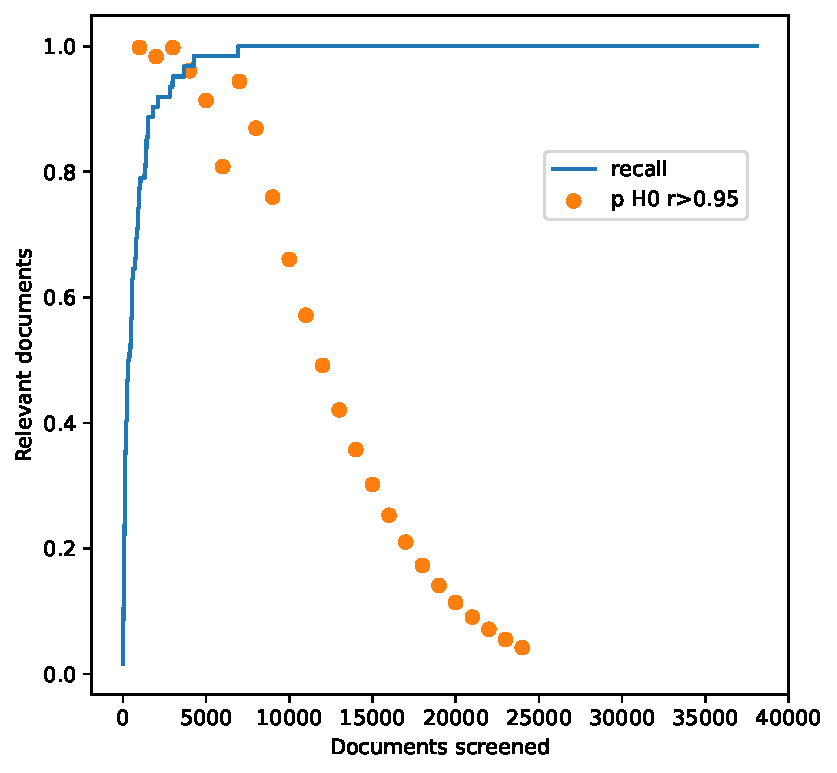
\includegraphics[width=\columnwidth]{../../figures/stopping.pdf}}
			\end{figure}
		\end{column}
	\end{columns}

\end{frame}

%	
%\begin{frame}
%	Thanks!
%	
%	\bigskip
%	
%	\hrule
%	
%	\bigskip
%	
%	\url{callaghan@mcc-berlin.net}
%	 
%	\medskip
%	
%	Twitter: @MaxCallaghan5
%	
%	\bigskip
%	
%	\begin{figure}
%	
\includegraphics[width=0.1\columnwidth]{images/wellcome-logo-black.eps}
%	\end{figure}
%\end{frame}
%	



\begin{frame}
	\bibliography{../LLMs}
\end{frame}

\end{document}